


\section{ Construir um sistema de controle físico }

 O sistema físico, ou protótipo, foi desenvolvido utilizando a placa de desenvolvimento da Texas Instruments, modelo $Tiva^{TM}$ TM4C123GH6PM, drive para acionamento do motor utilizando PWM, motor DC acoplado a um CD, com uma etiqueta, Figura \ref{fig:discoSensor}, para acionar o sensor óptico e servir de indicador para contagem de giros do motor. Fonte de alimentação chaveada de 12V 10W. A maior parte do sistema pode ser visto na Figura \ref{fig:discoSensorGeral} .



\begin{figure}[!htb]
\center
\subfloat[]{
	\label{fig:discoSensor}
	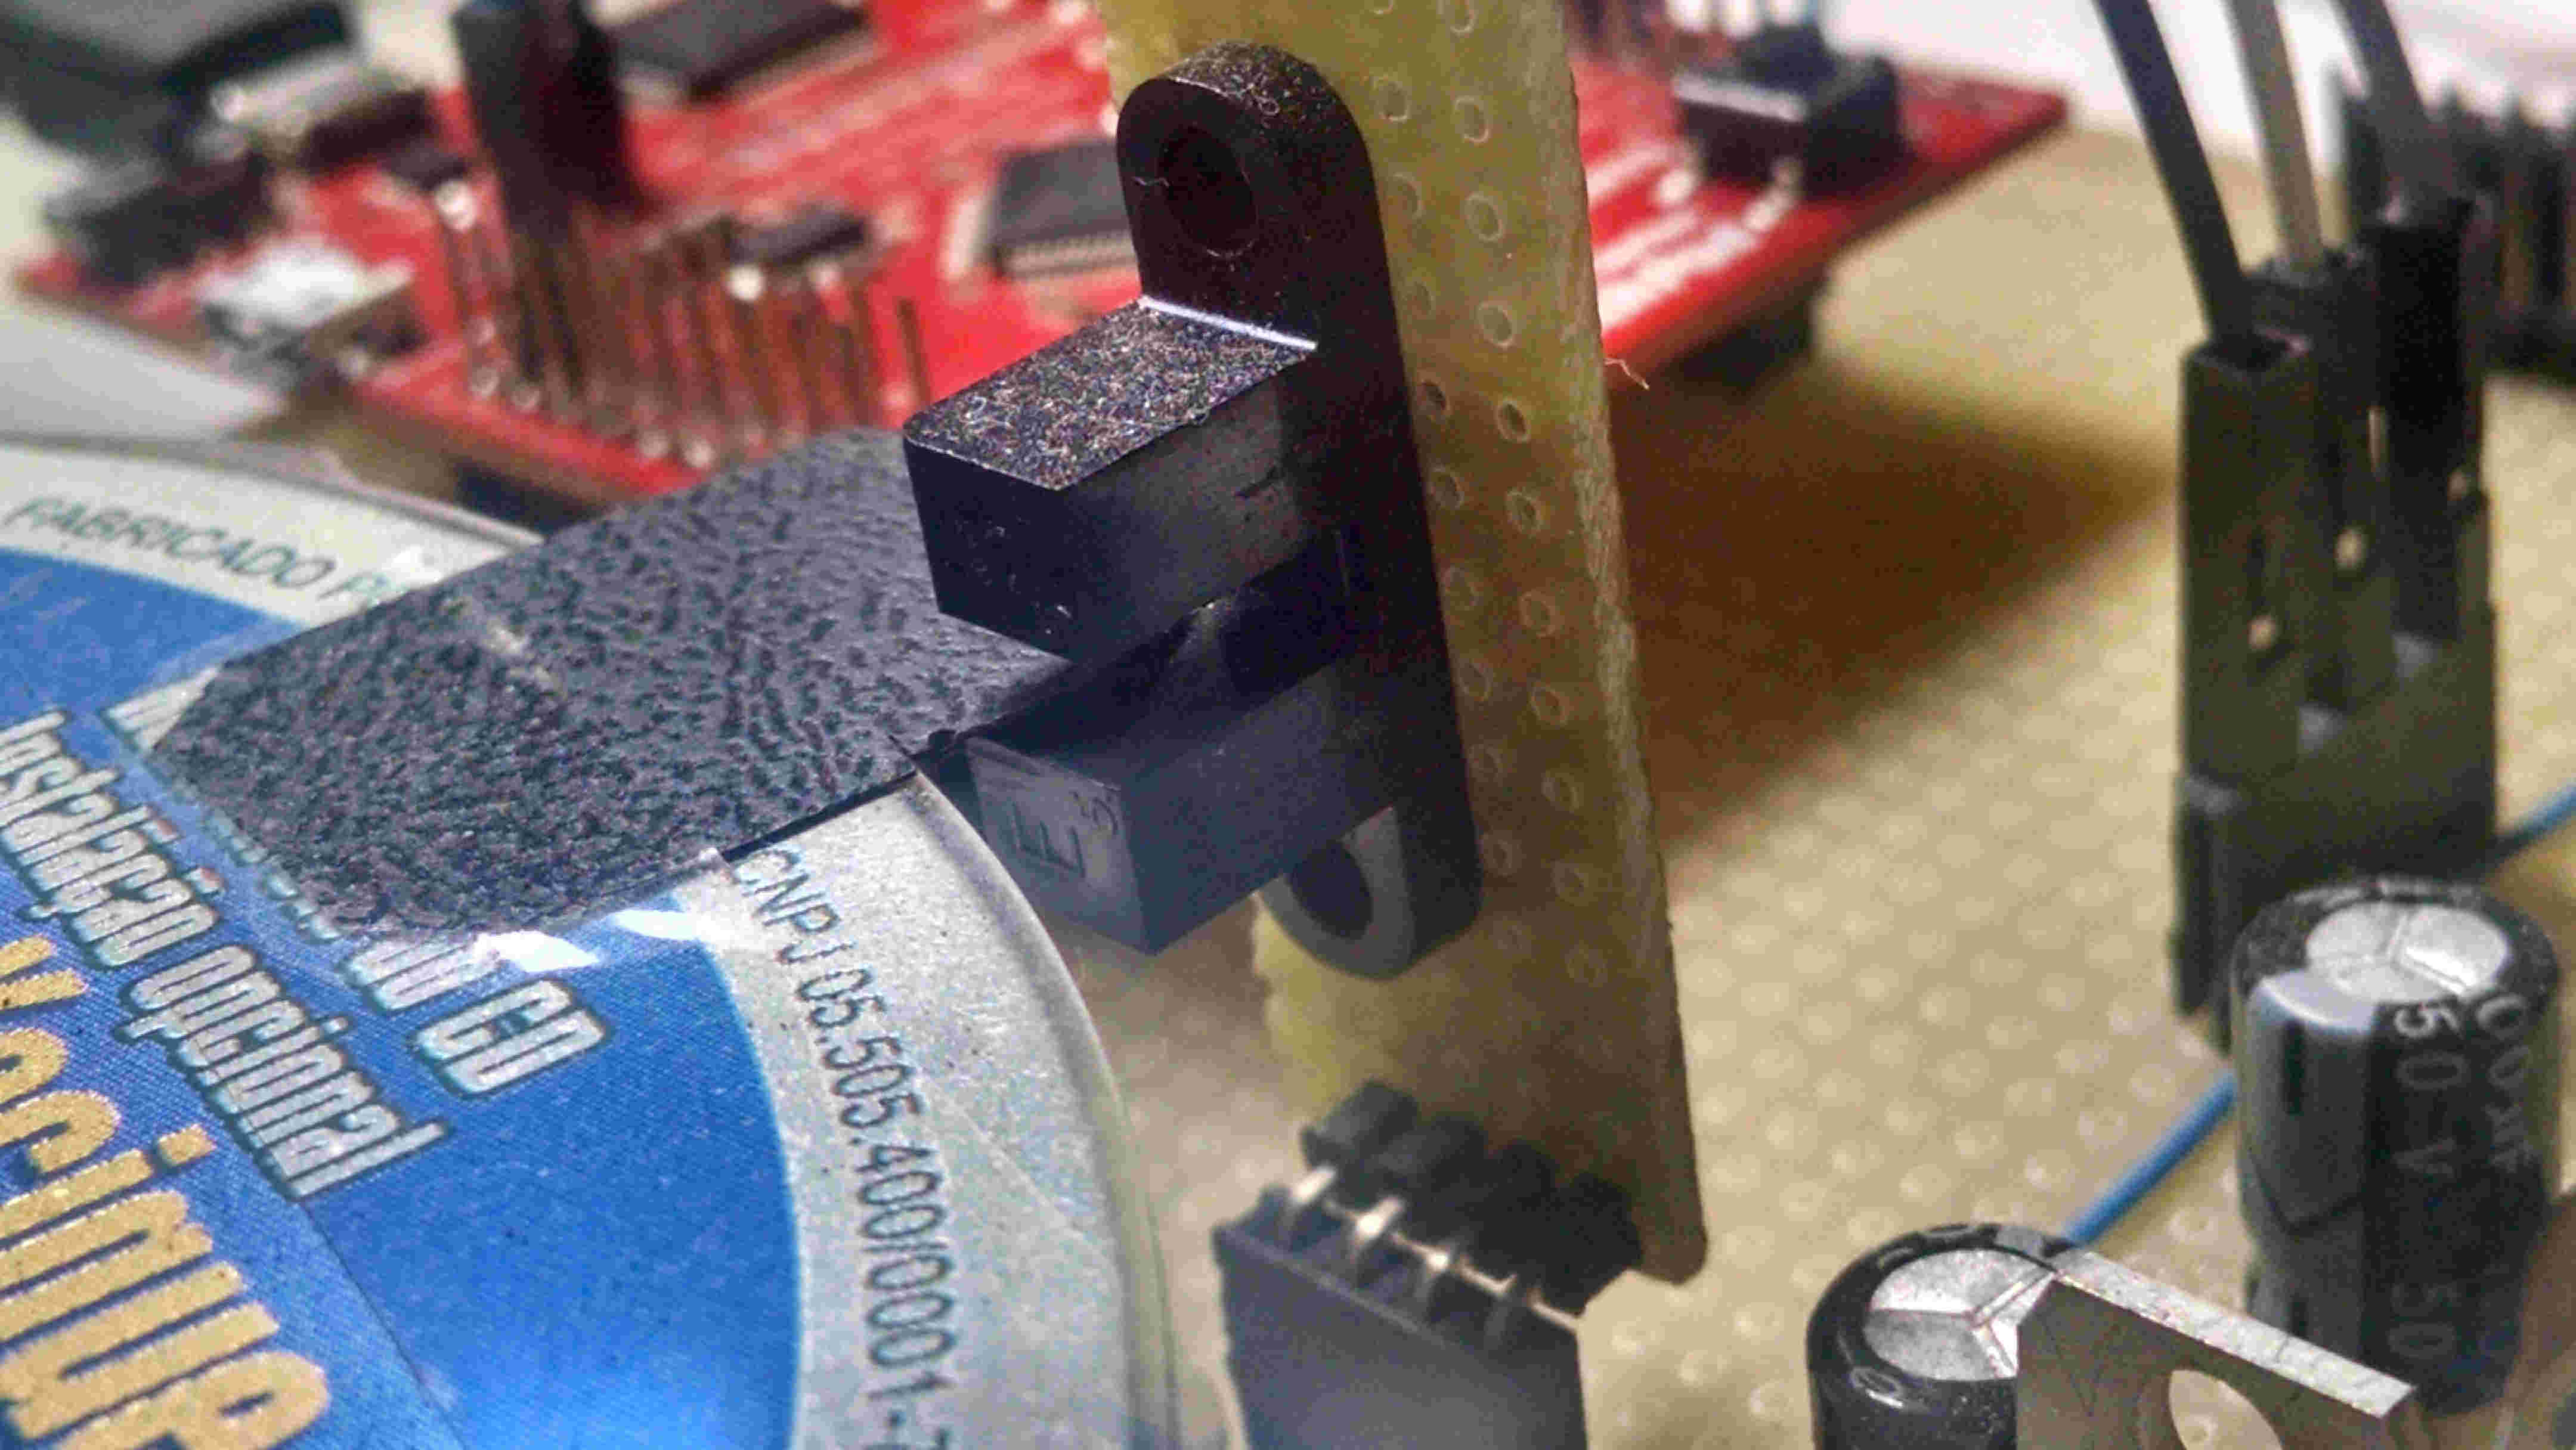
\includegraphics[scale=0.07, angle=0, clip=true, trim=300 200 1200 200]{./imagens/discoSensor.jpg}
	}
\subfloat[]{ 
	\label{fig:discoSensorGeral} 
	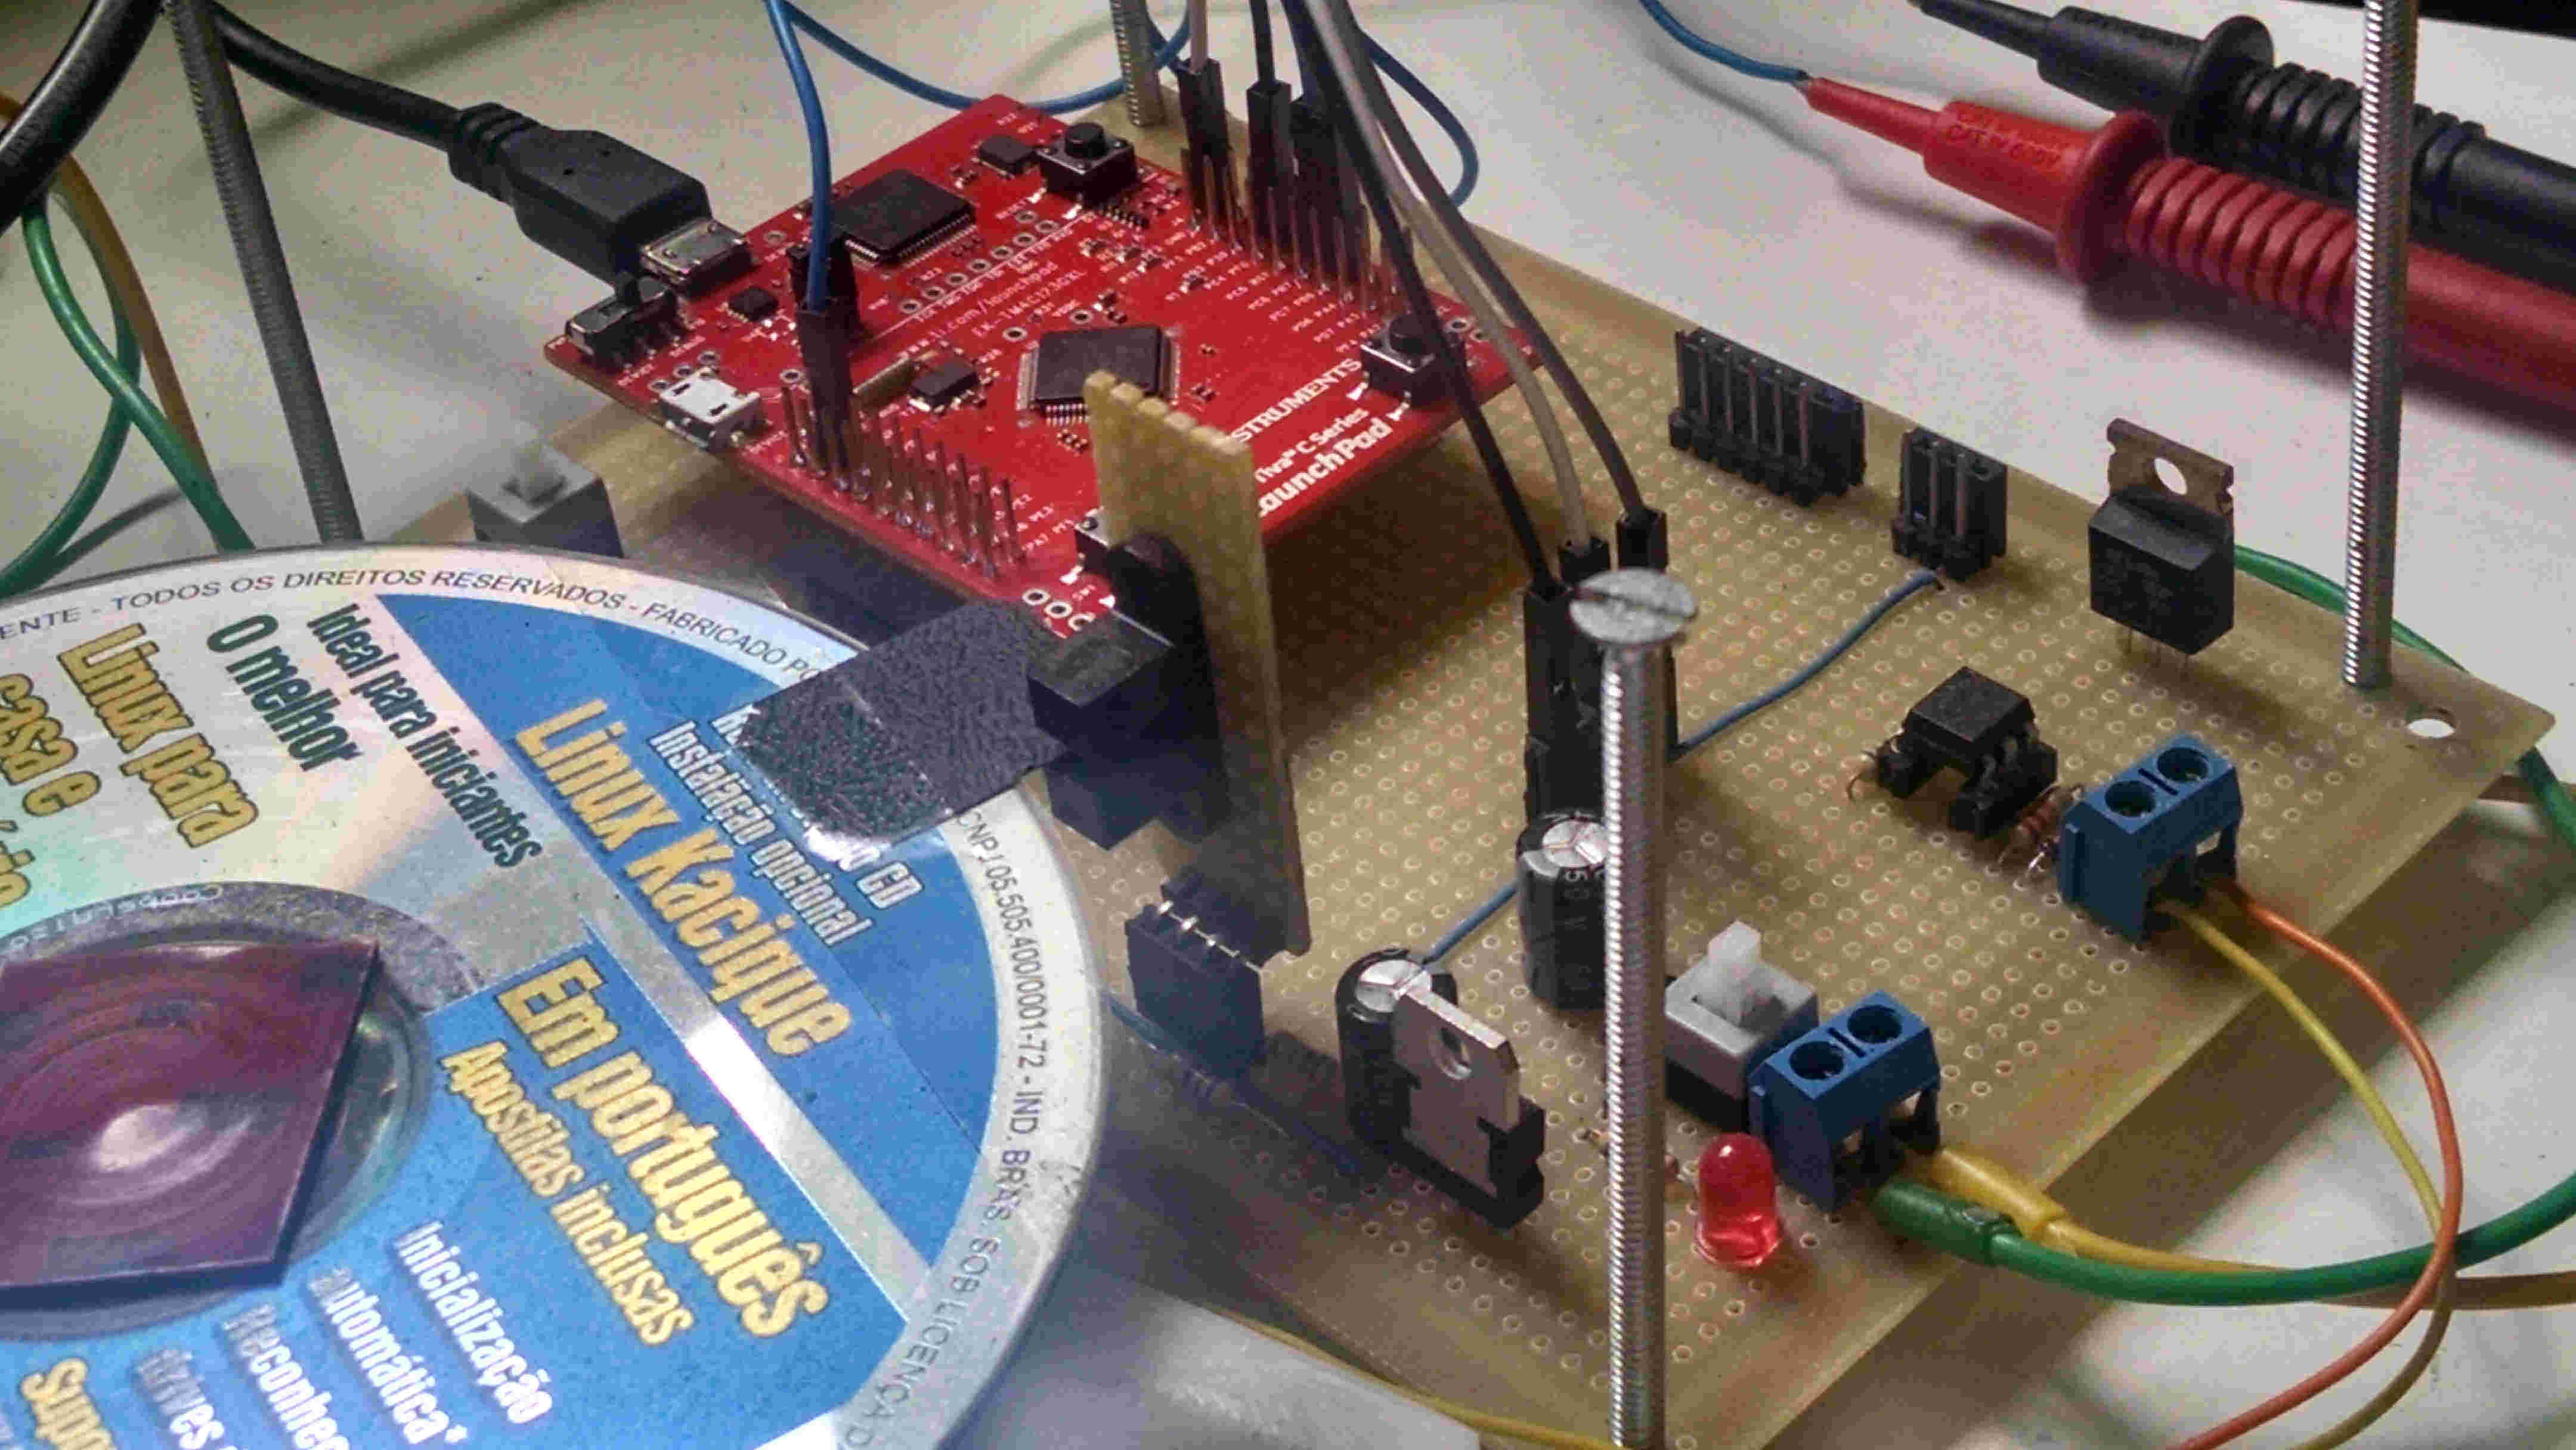
\includegraphics[scale=0.07, angle=0, clip=true, trim=300 200 400 200]{./imagens/discoSensorGeral.jpg} 
	}

\caption{Visão geral do sistema }
\end{figure}


\section{ Obter um modelo do processo }

Para melhor compreensão dos modelos dinâmicos dos sistemas, é utilizado o Diagrama de blocos do comportamento do sistema em malha aberta, conforme Figura \ref{fig:AcaoMalhaAberta}\cite{Ogata}.


\begin{comment}


\begin{figure}[!htb]
\centering
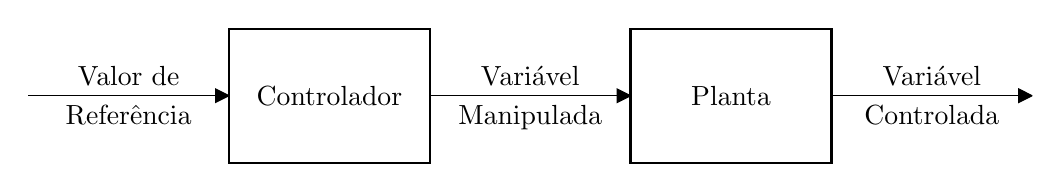
\begin{tikzpicture}[scale=0.85]
%\draw [lightgray](0,0) grid (15,2);
\draw (0,1) -- (3,1);
\draw [black, thick](3,0) rectangle (6, 2) ; 
\draw (6,1) -- (9,1);
\draw [black, thick](9,0) rectangle (12, 2) ; 
\draw (12,1) -- (15,1);

\draw [fill]( 3,1) -- ( 2.8, 1.1) -- ( 2.8,0.9) -- ( 3,1);
\draw [fill]( 9,1) -- ( 8.8, 1.1) -- ( 8.8,0.9) -- ( 9,1);
\draw [fill](15,1) -- (14.8, 1.1) -- (14.8,0.9) -- (15,1);

\node at ( 4.5, 1){Controlador};
\node at (10.5, 1){Planta};
\node [above] at ( 1.5,1){Valor de};
\node [below] at ( 1.5,1){Referência};
\node [above] at ( 7.5,1){Variável};
\node [below] at ( 7.5,1){Manipulada};
\node [above] at (13.5,1){Variável};
\node [below] at (13.5,1){Controlada};
\end{tikzpicture}
\caption{ Diagrama de blocos de sistema de controle em malha aberta}
\label{fig:malhaAberta}
\end{figure}

\end{comment}

Utilizando variáveis para cada elemento do Diagrama de blocos, de forma a representá-los nas equações, temos então que:



\begin{figure}[!htb]
\centering
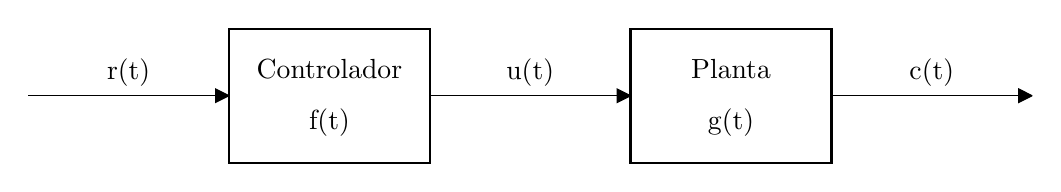
\begin{tikzpicture}[scale=0.85]
%\draw [lightgray](0,0) grid (15,2);
\draw (0,1) -- (3,1);
\draw [black, thick](3,0) rectangle (6, 2) ; 
\draw (6,1) -- (9,1);
\draw [black, thick](9,0) rectangle (12, 2) ; 
\draw (12,1) -- (15,1);

\draw [fill]( 3,1) -- ( 2.8, 1.1) -- ( 2.8,0.9) -- ( 3,1);
\draw [fill]( 9,1) -- ( 8.8, 1.1) -- ( 8.8,0.9) -- ( 9,1);
\draw [fill](15,1) -- (14.8, 1.1) -- (14.8,0.9) -- (15,1);

\node at ( 4.5, 1.4){Controlador};
\node at ( 4.5, 0.6){f(t)};
\node at (10.5, 1.4){Planta};
\node at (10.5, 0.6){g(t)};
\node [above] at ( 1.5,1){r(t)};
\node [above] at ( 7.5,1){u(t)};
\node [above] at (13.5,1){c(t)};
\end{tikzpicture}
\caption{ Sistema de controle em malha aberta}
\label{fig:AcaoMalhaAberta}
\end{figure}


Onde: 

%\begin{itemize}
%\item 
\hspace{1cm} $r(t)$: Valor de Referência em rotações por segundo [rps];

%\item 
$\hspace{1cm} f(t)$: Controlador que converte rps em \% PWM para acionar o motor;

%\item 
$\hspace{1cm} u(t)$: Variável Manipilada é o valor percentual do PWM;

%\item 
$\hspace{1cm} g(t)$: Planta ou Processo formado pelo motor DC com o disco acoplado no eixo;

%\item 
$\hspace{1cm}  c(t)$: Variável Controlada é a velocidade de rotação do eixo em rps.

%\end{itemize}



O sistema físico aqui estudado possui comportamento exponencial que pode ser descrito pela equação \ref{eq:ftSistOrdem1}. 






\begin{equation}
	 \frac{d c(t)}{dt} + c(t) = r(t) \rightarrow  \mathscr{L} \to \frac{C(s)}{R(s)} = \frac{K}{s + a} 
\label{eq:ftSistOrdem1}
\end{equation}

Onde:

\setlength{\parindent}{2cm}

$t$ : tempo,$ r(t) = 0$ , para t $<$ 0;

$\mathscr{L}$ : Operador de Laplace;

$c(t)$ : Variável controlada no domínio do tempo;

$C(s)$ : Variável controlada no domínio da frequência;

$r(t)$ : Valor de referência (\emph{setpoint}) no domínio do tempo;

$R(s)$ : Valor de referência (\emph{setpoint}) no domínio da frequência.

$K$ : Constante de proporcionalidade;

$s$ : Variável complexa de Laplace;

$a$ : Polo da função.
\setlength{\parindent}{0cm}



Sendo assim, para um estímulo de entrada do tipo \textbf{degrau}, com amplitude \textbf{A}, temos $ R(s) = \frac{A}{s}$ e aplicando a Transformada Inversa de Laplace:

\begin{equation}
C(s) = \frac{K}{s+a} \frac{A}{s} \rightarrow \mathscr{L}^{-1} \to c(t) = \frac{K A}{a} (1 - e^{-at})
\label{eq:degrauA}
\end{equation}

A Figura \ref{fig:degrauA} mostra um sinal do tipo degrau com amplitude \textbf{A} aplicado ao sistema de teste, que responde conforme um sistema de primeira ordem como mostrado na Figura \ref{fig:cRegime}. 


%A partir de um determinado instante de tempo, entra em regime constante ($c_{reg}$), alcançando o valor de referência dado pelo degrau de amplitude A. Assim quando $ t \rightarrow \infty $  então $ c_{reg} \rightarrow A $:




\begin{figure}[!htb]
\centering
\subfloat[Sinal de entrada tipo degrau com amplitude A]{\label{fig:degrauA}
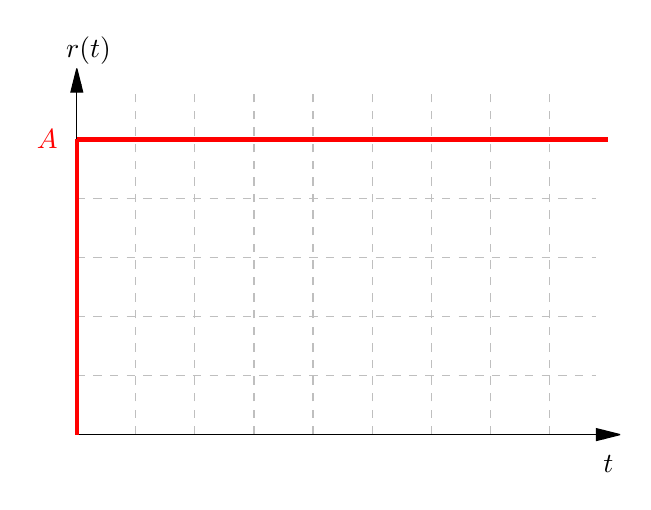
\begin{tikzpicture}[scale=0.75]
\draw [lightgray, dashed](0,0) grid (8.8,5.8);
\draw [->] (0,0) -- (9,0);
\draw [fill] (0,6.2) -- (-0.1, 5.8) -- (0.1,5.8) -- (0,6.2);
\draw [->] (0,0) -- (0,6);
\draw [fill] (9.2,0) -- (8.8,0.1) -- (8.8,-0.1)--(9.2,0.0);
\node at (9.0,-0.5) {$t$};
\node at (0.2,6.5) {$r(t)$};
\draw [red, ultra thick] (0.0,5.0) -- (9.0,5.0);
\draw [red, ultra thick] (0.0,0.0) -- (0.0,5.0);
\node at (-0.5,5.0)[red]{$A$};
\end{tikzpicture} }
\subfloat[Resposta transitória e regime de acomodação]{\label{fig:cRegime}
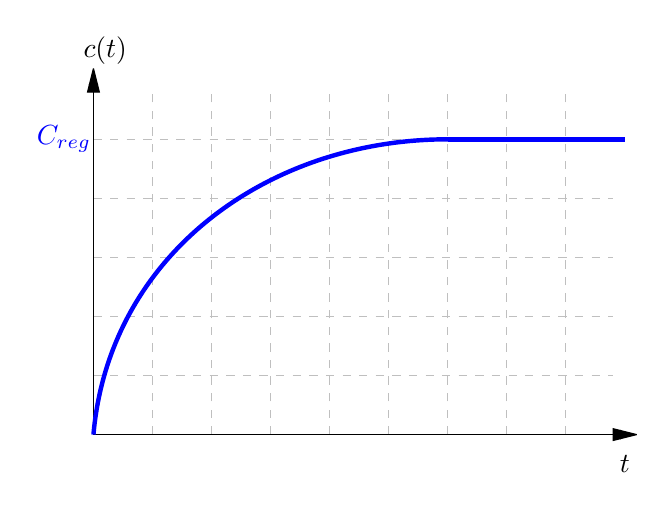
\begin{tikzpicture}[scale=0.75]
\draw [lightgray, dashed](0,0) grid (8.8,5.8);
\draw [->] (0,0) -- (9,0);
\draw [fill] (0,6.2) -- (-0.1, 5.8) -- (0.1,5.8) -- (0,6.2);
\draw [->] (0,0) -- (0,6);
\draw [fill] (9.2,0) -- (8.8,0.1) -- (8.8,-0.1)--(9.2,0.0);
\node at (9.0,-0.5) {$t$};
\node at (0.2,6.5) {$c(t)$};
\node at (-0.5,5.0)[blue]{$C_{reg}$};
\draw [blue, ultra thick] (0,0) to [out=85, in=180] (6,5);
\draw [blue, ultra thick] (6,5) -- (9,5);
\end{tikzpicture}}
\caption{Sistema de Primeira Ordem}
\label{fig:sistPrimeiraOrdem}
\end{figure}

%\begin{equation}
%c_{reg} = \lim_{t \rightarrow \infty} \frac{KA}{a}(1-e^{-at}) = \frac{KA}{a}
%\label{eq:cregime}
%\end{equation}



%Aplicando o Teorema do Valor Final pode-se ver que o \emph{$c_{reg}$} estabiliza em um valor constante como mostrado pela Equação \ref{eq:teoremaValorFinal}:

%\begin{equation}
%C_{reg} = \lim_{s \rightarrow 0} sC(s) = \lim_{s \rightarrow 0} s\ \frac{K}{s+a}\frac{A}{s} = \frac{KA}{a}
%\label{eq:teoremaValorFinal}
%\end{equation}



Matematicamente, quanto maior o valor de \emph{t} na Equação \ref{eq:degrauA}, o resultado da exponenencial tende a zero, levando a um resultado que depende apenas das constantes para o valor de referência. 

Tomando $t= \frac{1}{a} = a^{-1} = \tau$ para gerar um valor conhecido em $e^{-at}$, da Equação \ref{eq:degrauA} temos:


\begin{equation}
c(a^-1) = \frac{KA}{a}(1-e^{-(a.a^{-1})}) = \frac{KA}{a}(1-e^{-1}) = \frac{KA}{a}.0,63 = 0,63 . C_{reg}
\end{equation}

A Figura \ref{fig:constTempo} mostra a constante de tempo $\tau$, que é atingida quando o sistema alcança 63\% do seu valor de regime. Como sabemos que $\tau = \frac{1}{a}$, então o polo do sistema, que leva o denominador da Equação \ref{eq:degrauA} a zero, é:

\begin{equation}
a = \frac{1}{\tau}
\end{equation}



\begin{figure}
\centering
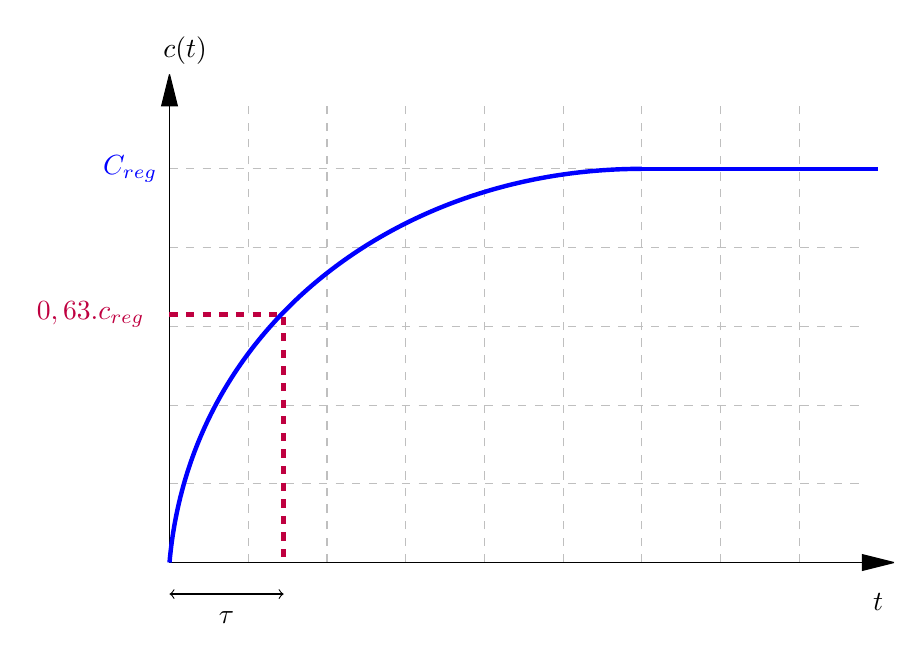
\begin{tikzpicture}[scale=1.0]
\draw [lightgray, dashed](0,0) grid (8.8,5.8);

\draw [->] (0,0) -- (9,0);
\draw [fill] (0,6.2) -- (-0.1, 5.8) -- (0.1,5.8) -- (0,6.2);
\draw [->] (0,0) -- (0,6);
\draw [fill] (9.2,0) -- (8.8,0.1) -- (8.8,-0.1)--(9.2,0.0);

\node at (9.0,-0.5) {$t$};
\node at (0.2,6.5) {$c(t)$};

\node at (-0.5,5.0)[blue]{$C_{reg}$};
\node at (-1,5.0*0.63)[purple]{$0,63.c_{reg}$};
\draw [purple, ultra thick, dashed] (0.0,5.0*0.63) -- (1.45,5.0*0.63)
						   -- (1.45,0.0);
\draw [blue, ultra thick] (0,0) to [out=85, in=180] (6,5);
\draw [blue, ultra thick] (6,5) -- (9,5);

\draw [<->] (0.0,-0.4) -- (1.45,-0.4); 
\node at (1.45/2,-0.7){$\tau$};

\end{tikzpicture}
\caption{Constante de tempo}
\label{fig:constTempo}
\end{figure}

Portanto:

\begin{equation}
K = \frac{ac_{reg}}{A}
\label{eq:calcK}
\end{equation}

%\begin{tikzpicture}
%\begin{axis}
%\addplot[title=Gráfico de uma função, 
%	xlabel = {$x$}, ylabel={$y$},
% 	red!70!blue, very thick, samples=200,
%	domain=-3:3]{x/(x^4-3*x^2+4)};
%\end{axis}
%\end{tikzpicture}



%\begin{figure}[!htb]
%\center	
%\includegraphics[scale=1.2]{./imagens/ftMalhaAberta.eps} 
%\label{fig:ftMalhaAberta} 
%\caption{ Função de Transferência empírica da planta}
%\end{figure}





A Figura \ref{fig:AcaoMalhaAberta} mostra um sinal do tipo degrau aplicado como referência no valor de \emph{25 rps}, a curva de comportamento real medida empiricamente e a curva aproximada calculada pelo método determinístico como segue:

\begin{figure}[!htb]
\center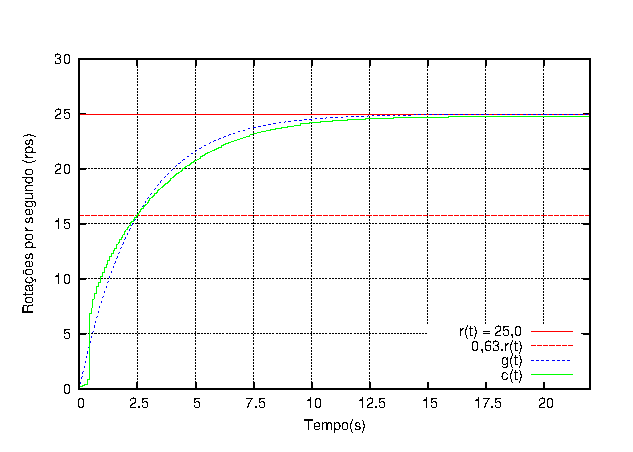
\includegraphics[scale=1.4]{./imagens/acaoMalhaAbertaTau.eps}
\caption{Ação de Controle em Malha Aberta}
\label{fig:acaoMalhaAberTau}
\end{figure}

A Figura \ref{fig:acaoMalhaAberTau} possui uma linha indicativa que mostra o ponto de intercepção da curva ao valor de 63\% do valor de referência, e empiricamente foi gerado um gráfico com divisões no eixo do Tempo no valor de $\tau = 2,5s $.

Calculando o polo da função:
\begin{equation}
  a = \frac{1}{\tau} = \frac{1}{2,5} = 0,4
\end{equation}

Como $c_{reg} = 25$ e $A$ também é $25$ então na Equação \ref{eq:calcK} $K = a$ e assim temos que:

\begin{equation}
c(t) = \frac{KA}{a}(1-e^{-at}) = \frac{0,4.25}{0,4}(1-e^{-0,4.t}) = 25(1-e^{-0.4.t})
\end{equation}


Aplicando a Transformada de Laplace:

\begin{equation}
  \frac{C(s)}{R(s)} = \frac{K}{s+a} = \frac{0,4}{s+0,4}
\end{equation}



Baseado no gráfico mostrado na Figura \ref{fig:acaoMalhaAberTau}, o valor de tempo em que o motor assume a velocidade de referência é aproximadamente $5\tau$, 12,5 s, e como objetivo para uma primeira versão da implementação do controle utilizando LPA2v é proposto que o sistema reduza o tempo de alcance da velocidade alvo em um tempo de no máximo $1\tau$, ou seja, $2,5 s$.


\subsection{ Qualidade do modelo }

A qualidade do modelo é relativa ao erro aceitável para o sistema estudado. Para o modelo obtido neste estudo foi aplicada o cálculo de Erro Relativo Percentual, e foram feitas análises em trechos diferentes em função da não linearidade inicial apresentada pelo comportamento do motor da planta em estudo.

A equação para o cálculo de Erro Relativo Percentual foi:

\begin{equation}
 \% erro = \frac{| \text{\emph{valor real}} -\text{\emph{valor calculado}} |}{\text{\emph{valor real}}} x 100
\end{equation}

Realizando a somatória para o cálculo de erro médio com todas as amostras aquisitadas: 

\begin{equation}
 \% erro = \frac{100}{N} . \sum_{n = 0,00}^{n=22,40} {\frac{| \text{\emph{r[n]}} -\text{\emph{c[n]}} |}{\text{\emph{r[n]}}} } 
\end{equation}


Onde:

\setlength{\parindent}{2cm}
r : valor real; 

c : valor calculado;

n : número da amostra aquisitada;

N : número total de amostras.

Obs.: As aquisições iniciaram com tempo inicial de 0,00 s até o tempo final de 22,40 segundos, com intervalo de 10 milisegundos entre aquisições, totalizando 2240 amostras.

\setlength{\parindent}{0cm}

A Tabela \ref{tab:ErroModelo} mostra o erro médio relativo calculado para diferentes intervalos de tempo. O primeiro valor contempla o intervalo completo de tempo amostrado, de 0,00 até 22,40 s com um erro de 10,77\%. Porém devido a não linearidade inicial, ocorre uma distorção bem grande que pode ser visto nos dois outros intervalos, de 0,00 a 0,50 segundos com erro de 364,13\%, completamente não aceitável, mas que após os 50 milisegundos iniciais, o erro médio é de 2.71\%. 


\begin{table}[h]
\centering
\caption{Erro Relativo Percentual}
\label{tab:ErroModelo}

\begin{tabular}{c|c}
\hline
Intervalo de amostras  &  erro médio relativo \\ \hline
\hline
0,00 a 22,40 s  &   10,77 \% \\ \hline
0,00 a  0,50 s 	&  364,13 \% \\ \hline
0,50 a 22,40 s  &    2,71 \% \\ \hline

\end{tabular}
\end{table}


De forma mais detalhada, 
foram calculados os erros médios relativos para cada intervalo de 
tempo de um $\tau$, 
e pode-se notar, 
pela Tabela \ref{tab:ErroModeloTau}, 
que o erro de estado estacionário, para o intervalo acima de 5 $\tau$, é menor do que 1\%. 


\begin{table}[h]
\centering
\caption{Erro Relativo Percentual para intervalos determinados por $\tau$ }
\label{tab:ErroModeloTau}

\begin{tabular}{c|c}
\hline
Intervalo de amostras  &  erro médio relativo \\ \hline
\hline
0 a 1 $\tau$ & 83,40 \% \\ \hline
1 a 2 $\tau$ &  3,16 \% \\ \hline
2 a 3 $\tau$ &  3,38 \% \\ \hline
3 a 4 $\tau$ &  2,00 \% \\ \hline
4 a 5 $\tau$ &  2,29 \% \\ \hline
$>$ 5 $\tau$ &  0,82 \% \\ \hline
\end{tabular}
\end{table}

O intervalo inicial, de 0 a 1$\tau$ apresenta um grande erro, devido a não linearidade já falada anteriormente, que ocorre no primeiros 50 ms. 




\begin{itemize}
\item Estudar a LPA2v;
\item Implementar um controlador utilizando LPA2v;
	\begin{itemize}
	\item Estabelecer a configuração do sistema;
	\item Descrever o controlador e parâmetros de ajuste;
	\end{itemize}
\item Otimizar parâmetros e analisar performance;
\end{itemize}



